\documentclass[journal,12pt,twocolumn]{IEEEtran}
\usepackage{setspace}
\usepackage{gensymb}
\usepackage{xcolor}
\usepackage{caption}
%\usepackage{subcaption}
%\doublespacing
\singlespacing
%\usepackage{graphicx}
%\usepackage{amssymb}
%\usepackage{relsize}
\usepackage[cmex10]{amsmath}
\usepackage{mathtools}
\usepackage{hyperref}
\usepackage{amsthm}
\usepackage{mathrsfs}
\usepackage{txfonts}
\usepackage{stfloats}
\usepackage{cite}
\usepackage{cases}
\usepackage{subfig}
%\usepackage{xtab}
\usepackage{longtable}
\usepackage{multirow}
%\usepackage{algorithm}
%\usepackage{algpseudocode}
%\usepackage{enumerate}
\usepackage{enumitem}
\usepackage{mathtools}
%\usepackage{iithtlc}
%\usepackage[framemethod=tikz]{mdframed}
\usepackage{listings}

%\usepackage{wasysym}
%\newcounter{MYtempeqncnt}
\DeclareMathOperator*{\Res}{Res}
%\renewcommand{\baselinestretch}{2}
\renewcommand\thesection{\arabic{section}}
\renewcommand\thesubsection{\thesection.\arabic{subsection}}
\renewcommand\thesubsubsection{\thesubsection.\arabic{subsubsection}}

\renewcommand\thesectiondis{\arabic{section}}
\renewcommand\thesubsectiondis{\thesectiondis.\arabic{subsection}}
\renewcommand\thesubsubsectiondis{\thesubsectiondis.\arabic{subsubsection}}

\hyphenation{op-tical net-works semi-conduc-tor}

\lstset{
language=Python,
frame=single, 
breaklines=true,
columns=fullflexible
}

\begin{document}

\theoremstyle{definition}
\newtheorem{theorem}{Theorem}[section]
\newtheorem{problem}{Problem}
\newtheorem{proposition}{Proposition}[section]
\newtheorem{lemma}{Lemma}[section]
\newtheorem{corollary}[theorem]{Corollary}
\newtheorem{example}{Example}[section]
\newtheorem{definition}{Definition}[section]
\newcommand{\BEQA}{\begin{eqnarray}}
\newcommand{\EEQA}{\end{eqnarray}}
\newcommand{\define}{\stackrel{\triangle}{=}}
\bibliographystyle{IEEEtran}
%\bibliographystyle{ieeetr}
\providecommand{\nCr}[2]{\,^{#1}C_{#2}} % nCr
\providecommand{\nPr}[2]{\,^{#1}P_{#2}} % nPr
\providecommand{\mbf}{\mathbf}
\providecommand{\pr}[1]{\ensuremath{\Pr\left(#1\right)}}
\providecommand{\qfunc}[1]{\ensuremath{Q\left(#1\right)}}
\providecommand{\sbrak}[1]{\ensuremath{{}\left[#1\right]}}
\providecommand{\lsbrak}[1]{\ensuremath{{}\left[#1\right.}}
\providecommand{\rsbrak}[1]{\ensuremath{{}\left.#1\right]}}
\providecommand{\brak}[1]{\ensuremath{\left(#1\right)}}
\providecommand{\lbrak}[1]{\ensuremath{\left(#1\right.}}
\providecommand{\rbrak}[1]{\ensuremath{\left.#1\right)}}
\providecommand{\cbrak}[1]{\ensuremath{\left\{#1\right\}}}
\providecommand{\lcbrak}[1]{\ensuremath{\left\{#1\right.}}
\providecommand{\rcbrak}[1]{\ensuremath{\left.#1\right\}}}
\theoremstyle{remark}
\newtheorem{rem}{Remark}
\newcommand{\sgn}{\mathop{\mathrm{sgn}}}
\providecommand{\abs}[1]{\left\vert#1\right\vert}
\providecommand{\res}[1]{\Res\displaylimits_{#1}} 
\providecommand{\norm}[1]{\lVert#1\rVert}
\providecommand{\mtx}[1]{\mathbf{#1}}
\providecommand{\mean}[1]{E\left[ #1 \right]}
\providecommand{\fourier}{\overset{\mathcal{F}}{ \rightleftharpoons}}
\providecommand{\ztrans}{\overset{\mathcal{Z}}{ \rightleftharpoons}}
%\providecommand{\hilbert}{\overset{\mathcal{H}}{ \rightleftharpoons}}
\providecommand{\system}{\overset{\mathcal{H}}{ \longleftrightarrow}}
	%\newcommand{\solution}[2]{\textbf{Solution:}{#1}}
\newcommand{\solution}{\noindent \textbf{Solution: }}
\providecommand{\dec}[2]{\ensuremath{\overset{#1}{\underset{#2}{\gtrless}}}}
\numberwithin{equation}{section}
%\numberwithin{equation}{subsection}
%\numberwithin{problem}{subsection}
%\numberwithin{definition}{subsection}
\makeatletter
\@addtoreset{figure}{problem}
\makeatother
\let\StandardTheFigure\thefigure
%\renewcommand{\thefigure}{\theproblem.\arabic{figure}}
\renewcommand{\thefigure}{\theproblem}
%\numberwithin{figure}{subsection}
\def\putbox#1#2#3{\makebox[0in][l]{\makebox[#1][l]{}\raisebox{\baselineskip}[0in][0in]{\raisebox{#2}[0in][0in]{#3}}}}
     \def\rightbox#1{\makebox[0in][r]{#1}}
     \def\centbox#1{\makebox[0in]{#1}}
     \def\topbox#1{\raisebox{-\baselineskip}[0in][0in]{#1}}
     \def\midbox#1{\raisebox{-0.5\baselineskip}[0in][0in]{#1}}
\vspace{3cm}
\title{Digital Signal Processing}
\author{sumeeth kumar} 
% make the title area
\maketitle
%\newpage
\tableofcontents
\renewcommand{\thefigure}{\theenumi}
\renewcommand{\thetable}{\theenumi}
%\renewcommand{\theequation}{\thesection}
\bigskip
\begin{abstract}
This manual provides a simple introduction to digital signal processing.
\end{abstract}
\noindent \section{Software Installation}
\noindent Run the following commands (commands may change depending on Linux distro)
\begin{lstlisting}
$ sudo apt update && sudo apt upgrade
$ sudo apt install libffi-dev libsndfile1 python3-scipy python3-numpy python3-matplotlib 
$ pip3 install cffi pysoundfile 
\end{lstlisting}
\section{Digital Filter}
\begin{enumerate}[label=\thesection.\arabic*
,ref=\thesection.\theenumi]
\item
\label{prob:input}
Download the sound file using
\begin{lstlisting}
$https://github.com/sumeethkumar12/signal-processing/blob/main/Sound_With_ReducedNoise.wav
\end{lstlisting}
\item
\label{prob:spectrogram}
You will find a spectrogram at \href{https://academo.org/demos/spectrum-analyzer}{\url{https://academo.org/demos/spectrum-analyzer}}. Upload the sound file that you downloaded in Problem \ref{prob:input} in the spectrogram and play. Observe the spectrogram. What do you find?
\solution There are a lot of yellow lines between 440 Hz to 5.1 KHz.  These represent the synthesizer key tones. Also, the key strokes
are audible along with background noise.
\item
\label{prob:output}
Write the python code for removal of out of band noise and execute the code.\\
\solution
Download the source code using
\begin{lstlisting}
$ https://github.com/sumeethkumar12/signal-processing/blob/main/codes/cancel_noise.py
\end{lstlisting}
and execute it using
\begin{lstlisting}
$ python3 cancel_noise.py
\end{lstlisting}
\item
The output of the python script in Problem \ref{prob:output} is the audio file \texttt{Sound\_With\_ReducedNoise.wav}. Play the file in the spectrogram in Problem \ref{prob:spectrogram}. What do you observe?\\
\solution The key strokes as well as background noise is subdued in the audio. Also, the signal is blank for frequencies above 5.1 kHz.
\end{enumerate}
\section{Difference Equation}
\begin{enumerate}[label=\thesection.\arabic*,ref=\thesection.\theenumi]
\item Let
\begin{equation}
x(n) = \cbrak{\underset{\uparrow}{1},2,3,4,2,1}
\end{equation}
Sketch $x(n)$.
\item Let
\begin{multline}
\label{eq:iir_filter}
y(n) + \frac{1}{2}y(n-1) = x(n) + x(n-2), 
\\
y(n) = 0, n < 0
\end{multline}
Sketch $y(n)$.\\
\solution The following code yields Fig. \eqref{fig:xnyn}.
\begin{lstlisting}
$ https://github.com/sumeethkumar12/signal-processing/blob/main/codes/xnyn.py
\end{lstlisting}
and execute it using
\begin{lstlisting}
$ python3 xnyn.py
\end{lstlisting}
\begin{figure}[!ht]
	\centering
	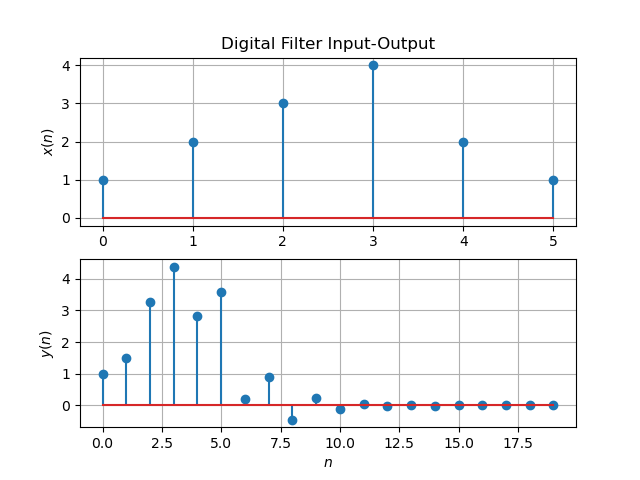
\includegraphics[width=\columnwidth]{xnyn.png}
	\caption{Plot of $x(n)$ and $y(n)$}
	\label{fig:xnyn}
\end{figure}
\item Repeat the above exercise using a C code.
\begin{lstlisting}
$ https://github.com/sumeethkumar12/signal-processing/blob/main/codes/xnyn.c
\end{lstlisting}

\end{enumerate}
\section{$Z$-transform}
\begin{enumerate}[label=\thesection.\arabic*]
\item The $Z$-transform of $x(n)$ is defined as 
%
\begin{equation}
\label{eq:z_trans}
X(z)={\mathcal {Z}}\{x(n)\}=\sum _{n=-\infty }^{\infty }x(n)z^{-n}
\end{equation}
%
Show that
\begin{equation}
\label{eq:shift1}
{\mathcal {Z}}\{x(n-1)\} = z^{-1}X(z)
\end{equation}
and find
\begin{equation}
	{\mathcal {Z}}\{x(n-k)\} 
\end{equation}
\solution Given that,
  \begin{align}
     X\brak{z} &= \mathcal{Z}\cbrak{x\brak{n}}\\
               &= \sum_{n = -\infty}^{\infty}x\brak{n}z^{-n}
  \end{align}
  So,
   \begin{align}
     \mathcal{Z}\cbrak{x\brak{n-1}} &= \sum_{n=-\infty}^{\infty}x\brak{n-1}z^{-n}
   \end{align}
   Take $k = n-1$,
   \begin{align}
           &= \sum_{k=-\infty}^{\infty}x\brak{k}z^{-\brak{k+1}}\\
           &= z^{-1}\sum_{k=-\infty}^{\infty}x\brak{k}z^{-k}\\
           &= z^{-1}\sum_{n=-\infty}^{\infty}x\brak{n}z^{-n}\\
           &= z^{-1}X\brak{z}    
   \end{align}
   resulting in $\eqref{eq:shift1}$ and similarly following the above steps you will get,
     \begin{align}
          \mathcal{Z}\cbrak{x\brak{n-k}} &= z^{-k}X\brak{n}\label{shift_k_Z_transform}
     \end{align} 
\item
   Now we will find $Z$ transform of the signal $x\brak{n}$,from $\eqref{xn}$,
    \begin{align}
      \mathcal{Z}\cbrak{x\brak{n}} &= \sum_{n=0}^{5}x\brak{n}z^{-n}\\
                                   &= 1z^{0} + 2z^{-1} + 3z^{-2}+4z^{-3} + 2z^{-4} +1z^{-5}\\
                                   &= 1 + 2z^{-1} + 3z^{-2} + 4z^{-3} + 2z^{-4} + z^{-5} 
    \end{align}
   \item Find
   %
   \begin{equation}
   H(z) = \frac{Y(z)}{X(z)}
   \end{equation}
   %
   from  $\eqref{eq:iir_filter}$ assuming that the $Z$-transform is a linear operation.
   \\
   \solution Applying \eqref{shift_k_Z_transform} in \eqref{eq:iir_filter},
   \begin{align}
   Y(z) + \frac{1}{2}z^{-1}Y(z) &= X(z)+z^{-2}X(z)
   \\
   \implies \frac{Y(z)}{X(z)} &= \frac{1 + z^{-2}}{1 + \frac{1}{2}z^{-1}}
   \label{eq:freq_resp}
   \end{align}
   %
    \solution 
     Now we will rewrite $\eqref{eq:iir_filter}$,
      \begin{align}
          y(n) + \frac{1}{2}y(n-1) = x(n) + x(n-2)
      \end{align}
     Now since $Z$-transform is a linear operator we can write that,
      \begin{align}
          Y\brak{n} + \frac{1}{2}Y\brak{n-1} &= X\brak{n} + X\brak{n-2}
      \end{align}
      From $\eqref{shift_k_Z_transform}$,
      \begin{align}
          Y\brak{n} + \frac{z^{-1}}{2}Y\brak{n} &= X\brak{n} + z^{-2}X\brak{n}\\
       \implies \frac{Y\brak{n}}{X\brak{n}} &= \frac{1 + z^{-2}}{1 + \frac{z^{-1}}{2}} 
      \end{align}       
      \item Find the Z transform of 
      \begin{equation}
      \label{delta}
      \delta(n)
      =
      \begin{cases}
      1 & n = 0
      \\
      0 & \text{otherwise}
      \end{cases}
      \end{equation}
      and show that the $Z$-transform of
      \begin{equation}
      \label{eq:unit_step}
      u(n)
      =
      \begin{cases}
      1 & n \ge 0
      \\
      0 & \text{otherwise}
      \end{cases}
      \end{equation}
      is
      \begin{equation}
      U(z) = \frac{1}{1-z^{-1}}, \quad \abs{z} > 1
      \end{equation}
      \solution 
      The $Z$-transform of $\delta{n}$ is,
      \begin{align}
          \mathcal{Z}\cbrak{\delta{n}} &= \sum_{n=-\infty}^{\infty}\delta\brak{n}z^{-n}\\
                                       &= \delta\brak{0}z^{0} + 0\,\, \brak{\text{Using \eqref{delta}}}\\
                                       &= 1
      \end{align}
       and the $Z$-transform of unit-step function $u\brak{n}$ is,
      \begin{align}
          U\brak{n} &= \sum_{n=-\infty}^{\infty}u\brak{n}z^{-n}\\
                    &= 0 + \sum_{n = 0}^{\infty}1.z^{-n}\\
                    &= 1 + z^{-1} + z^{-2} + .\,.\,.
      \end{align}
       Above is a infinite geometric series with $z^{-1}$ as common ratio , so we can write it as 
      \begin{align}
          U\brak{n} &= \frac{1}{1-z^{-1}} \because \abs{z} > 1
      \end{align} 
    \item Show that 
      \begin{equation}
        \label{eq:anun}
        a^nu(n) \ztrans \frac{1}{1-az^{-1}} \quad \abs{z} > \abs{a}
      \end{equation}
    \solution
     The $Z$- transform will be 
      \begin{align}
              \mathcal{Z}\cbrak{a^nu\brak{n}} &= \sum_{n = 0}^{\infty}a^{n}z^{-n}\\
                                              &= 1 + \frac{a}{z} + \brak{\frac{a}{z}}^2 + .\,.\,.\,.
      \end{align}
     Above is a infinite geometric series with first term $1$ and common ratio as $\frac{a}{z}$ and it can 
       be written as,
      \begin{align}
              \mathcal{Z}\cbrak{a^nu\brak{n}} &= \frac{1}{1 - \frac{a}{z}} \because \abs{a} < \abs{z} 
      \end{align}
     Therefore,
      \begin{equation}
          a^nu(n) \ztrans \frac{1}{1-az^{-1}} \quad \abs{z} > \abs{a}
      \end{equation}

\item
1et
\begin{equation}
H\brak{e^{\j \omega}} = H\brak{z = e^{\j \omega}}.
\end{equation}
Plot $\abs{H\brak{e^{\j \omega}}}$.  Comment.  $H(e^{\j \omega})$ is
known as the {\em Discret Time Fourier Transform} (DTFT) of $x(n)$.
\solution The following code plots Fig. \eqref{fig:H-w}.
\begin{lstlisting}
$ https://github.com/sumeethkumar12/signal-processing/blob/main/codes/dtft.py
\end{lstlisting}
The figure can be generated using
\begin{lstlisting}
$ python3 dtft.py
\end{lstlisting}
We observe that $\left|H\brak{e^{j\omega}}\right|$ is periodic with fundamental period 2$\pi$.
\begin{figure}[!ht]
	\centering
	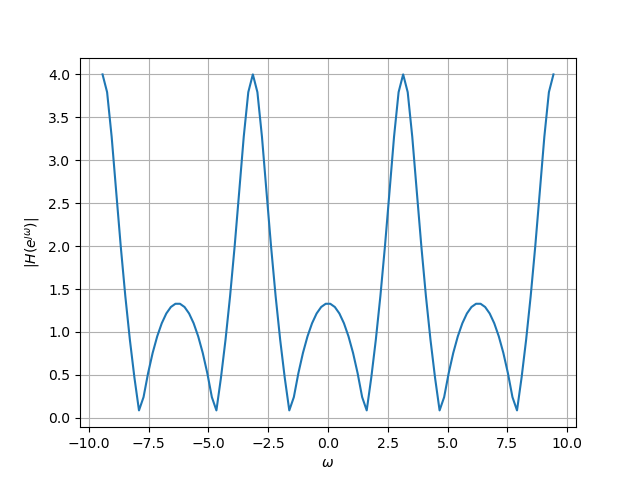
\includegraphics[width=\columnwidth]{dtft.png}
	\caption{Plot of $\left|H\brak{e^{j\omega}}\right|$ against $\omega$}
	\label{fig:H-w}
\end{figure}
Now using $\eqref{eq:freq_resp}$, we will find $\abs{H\brak{e^{j \omega}}}$,
     \begin{align}
      H\brak{e^{j \omega}} &= \frac{1+e^{-2j\omega}}{1 + \frac{e^{-j\omega}}{2}}\\
        \implies \abs{H\brak{e^{j \omega}}} &= \frac{\abs{1+e^{-2j\omega}}}{\abs{1 + \frac{e^{-j\omega}}{2}}}\\
                            &= \frac{\abs{1+e^{2j\omega}}}{\abs{e^{2j\omega} + \frac{e^{j\omega}}{2}}}\\
                            &= \frac{\abs{1+\cos2\omega + j\sin2\omega}}{\abs{e^{j\omega}+ \frac{1}{2}}}\\
                            &= \frac{\abs{4\cos^2\brak{\omega} + 4j\sin\brak{\omega}\cos\brak{\omega}}}{\abs{2e^{j\omega} + 1}}\\
                            &= \frac{\abs{4\cos\brak{\omega}}\abs{\cos\brak{\omega} + j\sin\brak{\omega}}}{\abs{2\cos\brak{\omega} + 1 + 2j\sin\brak{\omega}}}\\
        \therefore \abs{H\brak{e^{j \omega}}} &= \frac{\abs{4\cos\brak{\omega}}}{\sqrt{5 +4\cos\brak{\omega}}}
     \end{align}
      Using the above expression we can say that graph is symmetric about origin and has a period of $2\pi$.
  \item Express $h(n)$ in terms of $H\brak{e^{j \omega}}$.\\

	\solution 
	\begin{align}
		&\int_{-\pi}^{\pi} H(e^{\j\omega}) e^{\j\omega n} \der{\omega} \\
		&= \int_{-\pi}^{\pi} \sum_{k=-\infty}^\infty h(k)  e^{-\j\omega k} e^{\j\omega n} \der{\omega} \\
		&= \sum_{k=-\infty}^\infty h(k) \int_{-\pi}^{\pi} e^{\j\omega(n-k)} \der{\omega}
	\end{align}
	
	Now,
	\begin{align}
		 \int_{-\pi}^{\pi} e^{\j\omega(n-k)} \der{\omega} 
		 &= \begin{cases}
		 	\int_{-\pi}^\pi \der{\omega} & n-k = 0 \\
		 	\left.\frac{\exp\brak{\j\omega(n-k)}}{\j(n-k)}\right|_{-\pi}^\pi & n-k \ne 0
		 \end{cases} \\		 
		 &= \begin{cases}
		 	2\pi & n-k = 0 \\
		 	0 & n-k \ne 0
		 \end{cases} \\
		 &= 2\pi \delta(n-k)
	\end{align}
	
	Thus,
	\begin{align}
		\int_{-\pi}^{\pi} H(e^{\j\omega}) e^{\j\omega n} \der{\omega} &= 2\pi\sum_{k=-\infty}^\infty h(k) \delta(n-k) \\
		&= 2\pi h(n) * \delta(n) \\
		&= 2\pi h(n)
	\end{align}
	
	Therefore, $h(n)$ is given by the inverse DTFT (IDTFT) of $H\brak{e^{\j\omega}}$
	\begin{align}
		h(n) &= \frac{1}{2\pi} \int_{-\pi}^{\pi} H(e^{\j\omega}) e^{\j\omega n} \der{\omega} 
	\end{align}
\end{enumerate}

\section{Impulse Response}
\begin{enumerate}[label=\thesection.\arabic*]
\item \label{prob:impulse_resp}
Find an expression for $h(n)$ using $H(z)$, given that 
%in Problem \ref{eq:ztransab} and \eqref{eq:anun}, given that
\begin{equation}
\label{eq:impulse_resp}
h(n) \ztrans H(z)
\end{equation}
and there is a one to one relationship between $h(n)$ and $H(z)$. $h(n)$ is known as the {\em impulse response} of the
system defined by \eqref{eq:iir_filter}.
\\
\solution From \eqref{eq:freq_resp},
\begin{align}
H(z) &= \frac{1}{1 + \frac{1}{2}z^{-1}} + \frac{ z^{-2}}{1 + \frac{1}{2}z^{-1}}
\\
\implies h(n) &= \brak{-\frac{1}{2}}^{n}u(n) + \brak{-\frac{1}{2}}^{n-2}u(n-2)
\end{align}
using \eqref{eq:anun} and \eqref{eq:z_trans_shift}.
\item Sketch $h(n)$. Is it bounded? Convergent? 
\\
\solution The following code plots Fig. \ref{fig:h_n}.
\begin{lstlisting}
wget https://github.com/sumeethkumar12/signal-processing/blob/main/figs/h_n.png
\end{lstlisting}
Use the following command in the terminal to run the code
\begin{lstlisting}
python3 h_n.py
\end{lstlisting}
\begin{figure}[!ht]
\centering
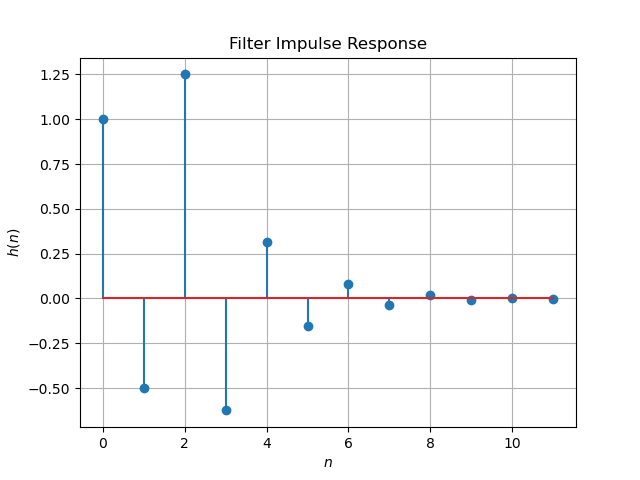
\includegraphics[width=\columnwidth]{h_n.png}
\caption{$h(n)$ as the inverse of $H(z)$}
\label{h_n.png}
\end{figure}
we can say it is bounded and convergent\\
\item The system with $h(n)$ is defined to be stable if
\begin{equation}
\sum_{n=-\infty}^{\infty}h(n) < \infty
\end{equation}
Is the system defined by \eqref{eq:iir_filter} stable for the impulse response in \eqref{eq:impulse_resp}?\\
\solution
\begin{align}
&u(n)=\begin{cases}
1 & n\geq 0\\
0 & n<0
\end{cases}\\
&u(n-2)=\begin{cases}
1 & n\geq 2\\
0 & n<2
\end{cases}\\
&\therefore h(n)=\begin{cases}
0 & n<0\\
\left(\frac{-1}{2}\right)^n & 0 \leq n<2\\
\left(\frac{-1}{2}\right)^n +\left(\frac{-1}{2}\right)^{(n-2)} & n \geq 2
\end{cases}\\
&\therefore \sum_{n=-\infty}^{\infty}h(n)=0+1+\frac{-1}{2}+\sum_{n=2}^{\infty}\left[\left(\frac{-1}{2}\right)^n +\left(\frac{-1}{2}\right)^{(n-2)}\right]\\
&=\frac{1}{2}+\frac{5}{4}*\left(\frac{2}{3}\right)=\frac{4}{3}<\infty\\
\end{align}
$\therefore$ system defined is stable
%
\item 
Compute and sketch $h(n)$ using 
\begin{equation}
\label{eq:iir_filter_h}
h(n) + \frac{1}{2}h(n-1) = \delta(n) + \delta(n-2), 
\end{equation}
%
This is the definition of $h(n)$.
\\
\solution The following code plots Fig. \ref{fig:hndef}. Note that this is the same as Fig. 
\ref{fig:hn}. 
%
\begin{lstlisting}
wget https://github.com/sumeethkumar12/signal-processing/blob/main/codes/hndef.py
\end{lstlisting}
Use the following command in the terminal to run the code
\begin{lstlisting}
python3 hndef.py
\end{lstlisting}
\begin{figure}[!ht]
\centering
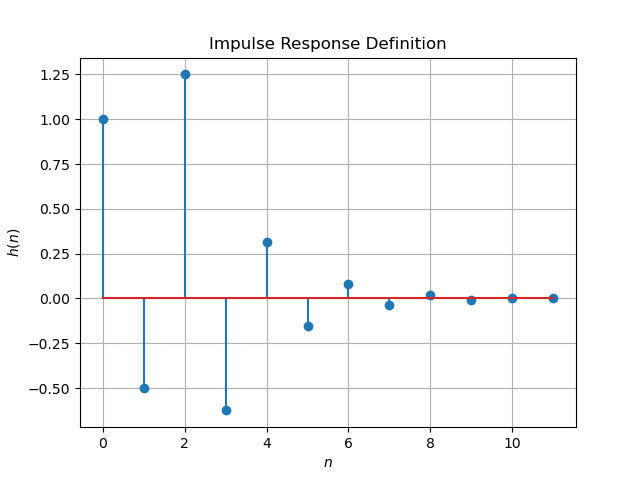
\includegraphics[width=\columnwidth]{hndef.png}
\caption{$h(n)$ from the definition}
\label{fig:hndef}
\end{figure}
%
\item Compute 
%
\begin{equation}
\label{eq:convolution}
y(n) = x(n)*h(n) = \sum_{k=-\infty}^{\infty}x(k)h(n-k)
\end{equation}
%
Comment. The operation in \eqref{eq:convolution} is known as
{\em convolution}.
%
\\
\solution The following code plots Fig. \ref{fig:ynconv}. Note that this is the same as 
$y(n)$ in  Fig. 
\ref{fig:xnyn}. 
%
\begin{lstlisting}
wget https://github.com/sumeethkumar12/signal-processing/blob/main/codes/ynconv.py
\end{lstlisting}
Use the following command in the terminal to run the code
\begin{lstlisting}
python3 ynconv.py
\end{lstlisting}
\begin{figure}[!ht]
\centering
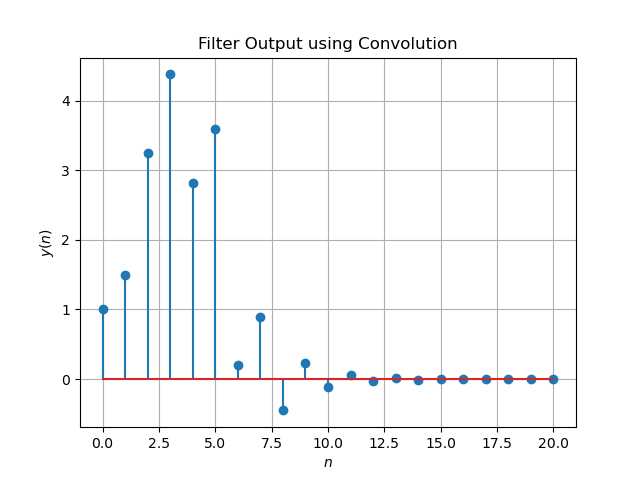
\includegraphics[width=\columnwidth]{ynconv.png}
\caption{$y(n)$ from the definition of convolution}
\label{fig:ynconv}
\end{figure}
\item Show that
\begin{equation}
y(n) =  \sum_{k=-\infty}^{\infty}x(n-k)h(k)
\end{equation}\\
\solution
wkt
\begin{align}
y(n) = x(n)*h(n) = \sum_{k=-\infty}^{\infty}x(k)h(n-k)
\end{align} 
Replacing $k$ with $n-k$
\begin{align}
=\sum_{n-k=-\infty}^{\infty}x(n-k)h(k)
\therefore y(n)=\sum_{k=-\infty}^{\infty}x(n-k)h(k)
\end{align}
\end{enumerate}
%
\end{document}
